% REMEMBER TO SET LANGUAGE!
\documentclass[a4paper,10pt, norsk]{article}
\usepackage[utf8]{inputenc}
\usepackage[norsk]{babel}
% Standard stuff
\usepackage{amsmath,graphicx,varioref,verbatim,amsfonts,geometry}
% colors in text
\usepackage[usenames,dvipsnames,svgnames,table]{xcolor}
% Hyper refs
\usepackage[colorlinks=false]{hyperref}

% Document formatting
\setlength{\parindent}{0mm}
\setlength{\parskip}{1.5mm}

%Color scheme for listings
\usepackage{textcomp}
\definecolor{listinggray}{gray}{0.9}
\definecolor{lbcolor}{rgb}{0.9,0.9,0.9}

%Listings configuration
\usepackage{listings}
%Hvis du bruker noe annet enn python, endre det her for å få riktig highlighting.

\lstdefinelanguage{python}
{
	morekeywords={print,abs,for,def,if,while,do,break,return,from,import,try,except,else,elif},
	sensitive=false,
	morecomment=[l]{\#}
}

\lstset{language=python,
	backgroundcolor=\color[rgb]{.95,.95,.95},
	numbers=left,xleftmargin=10pt,
	numberstyle=\tiny,stepnumber=1,numbersep=5pt,
	stringstyle=\color{red},
	basicstyle=\footnotesize \ttfamily,
	keywordstyle=\color{blue},
	commentstyle=\color{green},
	basewidth=0.60em,
	showstringspaces=false,
	captionpos=b,
	frame=single
}

\newcounter{subproject}
\renewcommand{\thesubproject}{\alph{subproject}}
\newenvironment{subproj}{
\begin{description}
\item[\refstepcounter{subproject}(\thesubproject)]
}{\end{description}}

%Lettering instead of numbering in different layers
% \renewcommand{\labelenumi}{\alph{enumi}}
\renewcommand{\thesubsection}{\alph{subsection}.}

%opening
\title{STK1100 - Oblig 1}
\author{William Dugan}

\begin{document}

\maketitle

\section{Oppgave 1}
\subsection{}
Vi får
\begin{align*}
    P(\text{5 forskjellige etasjer}) 
    = \frac{\text{gunstige utfall}}{\text{mulige utfall}} 
    = \frac{11*10*9*8*7}{11^5} 
    \approx 0.344.
\end{align*}

\subsection{}
Vi bruker $P(A') = 1 - P(A)$.
\begin{align*}
    P(\text{minst 2 i samme etasje})
    &= 1 - P(\text{ingen i samme etasje}) \\
    &= 1 - 0.344 \\
    &= 0.656.
\end{align*}

\subsection{}
Antall mulige ulike grupper på 3 som kan velges fra 5 personer kan skrives som
\begin{align*}
    \binom{5}{3} = 10.
\end{align*}

\subsection{}
Dersom systemet skal fungere, må enten 1 eller 2 fungere, eller (3 eller 4) og 5. Vi kaller undersystemet med komponent 1 og 2 for A og undersystemet med 3, 4, og 5 for B.
\begin{align*}
    P(1 \cup 2) 
    &= P(1) + P(2) - P(1 \cap 2) \\
    &= 0.9 + 0.9 - 0.9^2 \\
    &= 0.99
\end{align*}
Videre har vi $P(1\cup2) = P(3\cup4)$. Siden (3 og 4) og 5 er disjunkte  hendelser får vi
\begin{align*}
    P((3\cup4)\cap5) 
    &= P(3\cup4) * P(5) \\
    &= 0.99 * 0.9 \\
    &= 0.891
\end{align*}
Dermed får vi
\begin{align*}
    P(\text{Systemet funker})
    = P(A \cup B) 
    &= P(A) + P(B) - P(A \cap b) \\
    &= 0.99 + 0.891 - 0.99*0.891 \\
    &= \underline{\underline{0.9989}}.
\end{align*}

%\newpage
\section{Oppgave 2}
\subsection{}
For å løse denne oppgaven kan vi bruke Bayes' setning:
\begin{align}
    P(B_j | A) = \frac{P(A|B_j)P(B_j)}{\sum_{i=1}^{k} P(A|B_i)P(B_i)}
\end{align}

Dersom vi kaller hendingen A' for at Sara har glemt og mate fisken, og hendingen B for at gullfisken er død, får vi følgende uttrykk:
\begin{align*}
    P(A'|B)
    = \frac{P(B|A') P(A)}{P(B|A) P(A) + P(B|A') P(A')}
\end{align*}
hvor vi har brukt at utfallsrommet S = \{A, A'\}. Vi er gitt følgende sansynligheter:
\begin{align*}
    P(A) &= \frac{3}{4} \\
    P(A') &= \frac{1}{4} \\
    P(B|A) &= \frac{9}{10} \\
    P(B|A') &= \frac{1}{2}
\end{align*}
Setter vi dette inn i uttrykket vårt får vi at sannsynligheten for at Sara har glemt å mate fisken gitt at den er død etter ferien er \underline{\underline{0.469}}.

\newpage
\section{Oppgave 3}
\subsection{}
Fra definisjonen $P(A') = 1 - P(A)$ har vi
\begin{align*}
    F(x) 
    &= P(X \leq x) \\
    &= 1 - P(X > x)
\end{align*}
Videre må vi finne $P(X > x)$. Sannsynligheten for at en mann dør når han er n år gammel er $q_n$. Siden vi måler $X$ som levetid i hele år minus 35, får vi at sannsynligheten for at en mann skal dø når han er $X$ år er $q_{35+X}$. Dersom mannen skal leve til han er $n+1$ år, må han overleve det $n$-te året. Derfor får vi sannsynligheten for at han \textit{overlever} det $n$-te året lik $1-q_{35+n}$. Vi bruker at hendingen at mannen dør i år $n+1$ er disjunkt fra hendingen at han dør i år $n$. Dermed får vi produktet
\begin{align*}
    \prod_{n=0}^x (1 - q_{35+n})
\end{align*}
som er lik $P(X > x)$. Dermed får vi
\begin{align*}
    F(x)
    &= 1 - P(X > x) \\
    &= 1 - \prod_{n=0}^x (1 - q_{35+n})
\end{align*}
som var det vi skulle vise.

\subsection{}
Punktsannsynligheten i et punkt er gitt som hoppet i den kumulative fordelingsfunksjonen $F$. Dersom vi skal ha punktsannsynligheten i punkt $x$, må vi derfor trekke sannsynligheten i det foregående punktet fra sannsynligheten til $x$. Dermed får vi
\begin{align*}
    p(x)
    = P(X = x)
    = F(x) - F(x-1).
\end{align*}
siden vi måler $X$ i gjenstående levetid fra alder 35 er $x$ bare definert på intervallet $[0, 71]$. 

\subsection{}
Se \nameref{kode} for fullt program brukt.
\begin{figure}[h!]
        \centering 
        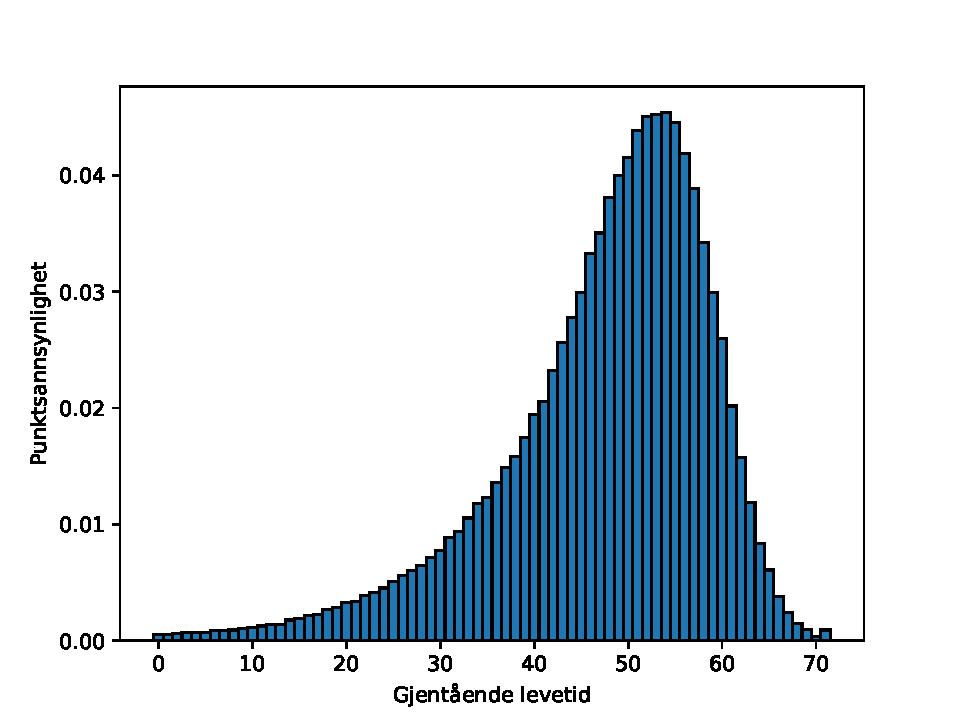
\includegraphics[scale=.85]{punktsannsynlighet.pdf} 
        \caption{Punktsannsynlighet $p_x$ for $x\in[0, 71]$.}
        \label{fig:px}
\end{figure}

\newpage
\subsection{}
Siden mannen ikke er pensjonist før han fyller 67 år, og X er gjenstående levetid, vil $h(X) = 0$ dersom $X \leq (66-35) = 31$. Hvis han blir 67 år eller eldre vil han få utbetalt 100 000 hvert år han lever etter fylte 67. Vi er gitt uttrykket for nåverdien til B som betales om k år er $B/1.03^k$. Dermed får vi for $X \geq 32$:
\begin{align*}
    h(X)
    = \sum_{k=32}^{X} \frac{10^5}{1.03^k}
\end{align*}
Vi kan trekke konstanten ut og skrive det resterende som summen av en geometrisk rekke, og får
\begin{align*}
    h(X)
    &= \frac{10^5}{1.03^{32}} * \sum_{k=32}^{X} \frac{1}{1.03^k} \\
    &= \frac{10^5}{1.03^{32}} * \sum_{k=1}^{X-31} \frac{1}{1.03^k} \\
    &= \frac{10^5}{1.03^{32}} * \frac{1-(1/1.03)^{X-31}}{1-(1/1.03)}
\end{align*}

\subsection{}
Fra formelheftet har vi forventningen for en reell funksjon $g(X)$ av en diskret stokastisk variabel $X$ er
\begin{align}
    E[g(X)] = \sum_j g(x_j)p(x_j)
\end{align}
hvor $j$ er domenet funksjonene er definert på. I vårt tilfelle er dette $n=0,1,\ldots, 71$. Vi har også $g(X)=h(X)$ som gir oss
\begin{align*}
    E[h(X)] = \sum_{x=0}^{71} h(x) p(x)
\end{align*}
hvor p(x) er punktsannsynligheten vi fant i oppg. b. Dette gir en forventet nåverdi av pensjonsutbetalinger på \underline{\underline{501 512 kr}}.

\subsection{}
Vi bruker samme tankegang som vi gjorde i oppg. d. Nåverdien av premieinnbetalingene er $K*B$, og $g(X)$ er summen av premieinnbetalingene. Den årlige premien $K$ er konstant, og vi trekker denne ut av summen. Videre må vi velge grensene til summen: Han starter betalingene når han fyller 35 år (X=0) og slutter enten når han fyller 66 (X=31), eller ved X=x hvis han dør tidligere. Vi velger derfor min(X, 31). Dermed får vi
\begin{align*}
    g(X) 
    = \sum_{k=0}^{\text{min}(X, 31)} \frac{1}{1.03^k} 
    = \frac{1-(1/1.03)^{X-31}}{1-(1/1.03)} 
\end{align*}

\subsection{}
Forventet nåverdi av mannens samlede premieinnbetalinger er $K*E[g(X)]$. Resultatet følger fra oppg. f ved å bruke samme logikk som oppg. e. Dette gir $E[g(X)] = \underline{\underline{20.60}}$.

\subsection{}
Siden
\begin{align*}
    K * E[g(X)] = E[h(X)]
\end{align*}
får vi
\begin{align*}
    K 
    = \frac{E[h(X)]}{E[g(X)]} 
    = \underline{\underline{24 341}}kr.
\end{align*}

\newpage
\section{Python-kode} \label{kode}
\lstinputlisting{oblig1_vektorisert.py}

\end{document}
